% vim: set fileencoding=utf-8 encoding=utf-8:
\documentclass[spanish]{article}
\usepackage{babel}
\usepackage[utf8]{inputenc}
\usepackage{fullpage}
\usepackage{url}
\usepackage{palatino}
\usepackage{amsmath}
\usepackage{amssymb}
\usepackage{graphicx}


\title{Reconocimiento de Patrones---Discusión del artículo \textit{Similarity~Measures}}
\author{Roberto Bonvallet \\ \url {<rbonvall@gmail.com>}}
\date{Agosto de 2008}

\begin{document}
\maketitle

\section{Resumen}
El artículo \textit{Similarity Measures}~\cite{sim} aborda el problema de medir
disimilaridades en espacios de características, desde el punto de vista de los
requerimientos de un sistema de recuperación de información.


\section{Modelos axiomáticos presentados en el artículo}
\subsection{Axiomas métricos}

\begin{description}
    \item [autosimilaridad constante:]
        $d(A, A) = d(B, B)$;
    \item [minimalidad:]
        $d(A, B)\ge d(A, A)$;
    \item [simetría:]
        $d(A, B) = d(B, A)$;
    \item [desigualdad triangular:]
        $d(A, B) + d(B, C)\ge d(A, C)$.
\end{description}
Muchos modelos de similaridad suponen que el espacio subyacente cumple con estos axiomas,



\subsection{Estructura de proximidad monótona}
\begin{description}
    \item [dominancia:]
        análoga a la desigualdad triangular, pero a lo largo de los ejes;
    \item [consistencia:]
        el orden a lo largo de una dimensión es independiente de otras
        dimensiones;
    \item [transitividad:]
        traslapes de trios ordenados inducen un orden más general;
    \item [desigualdad de esquina;]
\end{description}


\subsection{Modelo de contraste de características (FCM)}
\begin{description}
    \item [calce:]
    \item [monotonía:]
    \item [independencia:]
\end{description}

\subsection{FCM difuso con dependencia de características}


\section{Similaridad y recuperación de información}


\begin{itemize}
    \item recuperar elementos de una base de datos que son descripciones
        incompletas o esbozos de los elementos buscados;
    \item correlación con la similaritud perceptual.
    \item importancia de las características por separado.
    \item relevancia empíricamente observable
    \item comparación consulta-resultado en vez de punto-punto
\end{itemize}



\section{Modelos presentados}
\subsection{Métricos}





% set members for next example
\newcommand{\SMA}{\Box}
\newcommand{\SMB}{\spadesuit}
\newcommand{\SMC}{\heartsuit}
\newcommand{\SMD}{\clubsuit}
\newcommand{\SME}{\diamondsuit}

\begin{align*}
    A &= \{\phantom{\SMA,  \SMB,} \SMC,          \SMD,          \SME\}  \\
    B &= \{\phantom{\SMA,} \SMB,  \SMC,          \SMD\phantom{, \SME}\} \\
    C &=          \{\SMA,  \SMB,  \SMC\phantom{, \SMD,          \SME}\} \\
\end{align*}

\begin{figure}[t]
  \centering
  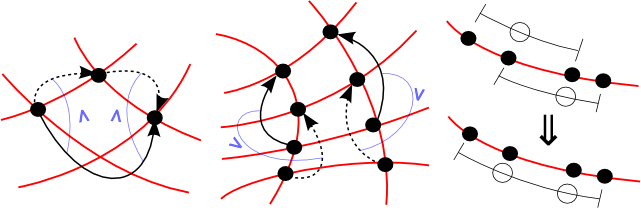
\includegraphics[bb=0 0 513 166]{imagenes/dom-cons-trans.png}
  % dom-cons-trans.png: 641x208 pixel, 90dpi, 18.09x5.87 cm, bb=0 0 513 166
  \caption{\small %
    Ejemplos de las propiedades de un espacio con estructura de proximidad
    monótona. Las líneas con flechas representan distancias entre puntos del
    espacio de características.
    (a) Dominancia: distancia diagonal es mayor que a lo largo de cada eje.
    (b) Consistencia: las relaciones de orden a lo largo de una dimensión son
        independientes de otras dimensiones.
    (c) Transitividad: relaciones de orden traslapadas fuerzan las mismas
        relaciones entre los puntos en la región de traslape.
  }
  \label{fig:cons-dom-trans}
\end{figure}

\begin{figure}[t]
  \centering
  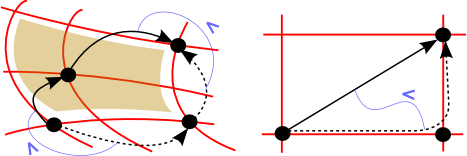
\includegraphics[bb=0 0 374 125]{imagenes/esquina.png}
  % esquina.png: 467x156 pixel, 90dpi, 13.18x4.40 cm, bb=0 0 374 125
  \label{fig:esquina}
  \caption{\small %
    Comparación entre la desigualdad de esquina y la desigualdad
    triangular.  La desigualdad triangular compara la distancias directa con
    la distancia a lo largo de dimensiones entre dos puntos.  La desigualdad de
    esquina sólo impone estas restricciones por tramos, pero deben cumplirse
    para cualquier lugar de la zona sombreada donde esté el punto central.
  }
\end{figure}




%\begin{thebibliography}{1}
\begin{thebibliography}{99}
    \bibitem{sim}
        Simone Santini, Ramesh Jain.
        \emph{Similarity Measures.}
        IEEE Trans.~on Pattern Analysis and Machine Inteligence.
        Vol.~21, No.~9, September~1999.
    \bibitem{shepard}
        Roger~{}N.~Shepard.
        \emph{Toward a Universal Law of Generalization for Physical Science.}
        Science, vol.~237, pp.~1317--1323, 1987.
\end{thebibliography}

\end{document}
